\documentclass[a4paper,12pt]{scrartcl}[1970/01/01]
\usepackage[ngerman]{babel}
\usepackage[T1]{fontenc}
\usepackage[utf8]{inputenc}
\usepackage{graphicx}
\usepackage{url}
\usepackage{cite}
\usepackage{float}
\usepackage{xcolor}
\usepackage[breaklinks=true]{hyperref}
	\definecolor{mygray}{RGB}{240,240,240}
	\definecolor{mywhite}{RGB}{255,255,255}
	\hypersetup{citebordercolor=mywhite,
				filebordercolor=mywhite,
				linkbordercolor=mywhite,
				menubordercolor=mywhite,
				urlbordercolor=mygray,
				runbordercolor=mywhite}
\usepackage{listings}

\title{Mobile Roboter SS12\\Gruppe 01}
\author{Kevin Walter, Gerhard Klostermeier, Andreas Jansche}
\date{\copyright\space\today}

\begin{document}
\maketitle
\newpage

\tableofcontents
\newpage

%%%Abschnitt:
%\section{Foo}
%\subsection{SubFoo}
%\subsection{Another SubFoo}
%%Ende Foo
%\newpage

%%%Bild:
%\begin{figure}[htbp]
%\centering
%\includegraphics{bilder/foo}
%\caption{This is a foo}
%\end{figure}

\section{Einleitung}
\subsection{Inhalte und Ziele}
Im Rahmen der Vorlesung "'Mobile Roboter"' der Hochschule Aalen wurden die Aufgaben aus dem Vorlesungsskript sowie eine größere, selbst ausgewählte Aufgabe bearbeitet.
Genutzt wurde Eclipse zum Entwickeln der Programme sowie avrdude zum Flashen des Microcontrollers des ct-Bot.

\subsection{Der ct-Bot}
"`Der c't-Bot ist ein Projekt der Fachzeitschrift c't aus dem Verlag Heinz Heise.
Er soll möglichst vielen Lesern den Zugang zu dem spannenden Thema Robotik eröffnen.
Daher besteht das Projekt aus zwei Teilen: Dem eigentlichen Roboter c't-Bot und dem passenden Simulator c't-Sim.

Den c't-Bot gibt es nur als Bausatz. In der Grundversion besitzt er zwei Räder,
hat eine runde Grundfläche vom Durchmesser einer CD und ist mit einer ganzen Reihe von Sensoren
bestückt. Seine Intelligenz sitzt in einem Mikrocontroller, der in C programmiert wird. Mechanik
und Intelligenz sind ein Tradeoff zwischen Preis, Eleganz und Stabilität. Ganz bewusst kommen keine
SMD-Bauteile zum Einsatz, damit auch unerfahrene Löter eine Chance haben,
sich ihren Spielgefährten aufzubauen.

Der Simulator c't-Sim ist in Java geschrieben und macht ausführlichen Gebrauch von der
3D-Bibliothek Java3D. Er läuft derzeit unter Windows und Linux. Damit man den ganzen Steuer-Code
für den Roboter nur einmal entwicklen muss, ist dieser in C geschrieben. Er läst sich für PC und Mikrocontroller
übersetzen. Auf dem PC nimmt er per TCP/IP Kontakt zum Simulator auf. Dieser versorgt den C-Teil dann mit Sensorwerten.
Auf dem Mikrocontroller liest er dann die echten Sensoren aus. Der Simulator funktioniert auch
ohne den Roboter und der Roboter auch ohne den Simulator.

Das ganze Projekt lebt vom Mitmachen. Der von c't vorgestellte Quelltext liefert zwar ein recht
vollständiges Framework für den Roboter und den Simulator, die Intelligenz des Roboters zu
implementieren bleibt aber den Lesern überlassen. Dennoch fließen pfiffge Patches immer wieder in
den offiziellen Code ein. Der gesamte Code steht unter der GPL."'
\footnote{Quelle: Benjamin Benz, \url{http://wiki.ctbot.de/index.php?title=Hauptseite&oldid=3655}}




%Ende Einleitung
\newpage

\section{Installation und Inbetriebnahme}
\subsection{Installation}
Für die Entwicklung wurden ein aktuelles Ubuntu Linux sowie ein Arch Linux verwendet. In diesem Abschnitt ist beschrieben was für vorbereitende Schritte auf dem System durchgeführt werden müssen um entwickeln und den ct-Bot flashen zu können.
(Die nachfolgenden Anweisungen gelten für Ubuntu.)


\subsubsection{System vorbereiten}
Zunächst müssen einige Softwarepakete nachinstalliert werden:
\begin{itemize}
\item eclipse-cdt\\
Die Eclipse-Variante zur C/C++-Entwicklung. (Der ct-Bot wird in C programmiert.)
\item binutils-avr, gcc-avr, avr-libc\\
Werden zum Kompilieren für den Microcontrollers des ct-Bot benötigt. (Cross-Compiler)
\item avrdude\\
Wird zum Flashen des Microcontroller des ct-Bot benötigt.
\item subversion\\
Wird zum Holen des aktuellen Quellcodes für den ct-Bot aus dem heise-Repository benötigt.
\end{itemize}
Der konkrete Befehl um die Pakete unter Ubuntu zu installieren sieht folgendermaßen aus:
\begin{lstlisting}
	sudo apt-get install eclipse-cdt binutils-avr gcc-avr \
	avr-libc avrdude subversion
\end{lstlisting}


\subsubsection{Quellcode holen}
Für den Quellcode erstellen wir zunächst ein Verzeichnis \textit{ctbot} und wechseln hinein:
\begin{lstlisting}
	mkdir ctbot && cd ctbot
\end{lstlisting}
Nun holen wir uns den aktuellen stable-Code vom heise-Repository:
\begin{lstlisting}
	svn checkout https://www.heise.de:444/svn/ctbot/stable
\end{lstlisting}
Der aktuelle Quellcode des ct-Bot befindet sich nun also unter \textit{\~{}/ctbot/stable} und muss im nächsten Schritt nur noch in Eclipse eingebunden werden.


\subsubsection{Eclipse einrichten}
Zunächst müssen wir den Quellcode in Eclipse einbinden:
\begin{itemize}
\item Dazu wählen wir zunächst im Menü \textit{File} den Unterpunkt \textit{Import}.
\item Dort wählen wir \textit{General -> Existing Projects into Workspace} und bestätigen mit \textit{Next >}.
\item Unter der Auswahl \textit{Select root directory} geben wir entweder direkt das Quellcodeverzeichnis an (\textit{\~{}/ctbot/stable/ct-Bot}) oder wählen das Verzeichnis über \textit{Browse...}.
\end{itemize}
Nun ist der Quellcode als Projekt in Eclipse eingebunden. Um für den ct-Bot zu kompilieren muss jedoch noch die Build-Configuration angepasst werden:
\begin{itemize}
\item Auf der linken Seite wählen wir zunächst das Projekt \textit{ct-Bot} aus.
\item Im Menü \textit{Project} wählen wir \textit{Properties} und dort \textit{C/C++-Build}.
\item Dort gehen wir auf \textit{Manage Configurations...} und wählen die Konfiguration \textit{Debug-MCU-m32}. Mit dieser Konfiguration wird der zuvor installierte Cross-Compiler genutzt um eine hex-Datei zum Flashen des ct-Bot zu erstellen.
\item Wir bestätigen die Auswahl der Konfiguration mit \textit{Set active} und verlassen die Einstellungen mit \textit{Ok}, \textit{Apply} und nochmals \textit{Ok}.
\end{itemize}
Nachdem nun auch die passende Konfiguration gewählt wurde lässt sich das Projekt nun auch kompilieren. Jedoch kommt es zu einigen Warnmeldungen.
Um diese Warnungen loszuwerden öffnen wir die Datei \textit{ct-Bot.h} (\textit{include/ct-Bot.h}) und suchen die Zeile
\begin{lstlisting}
//#define SPEED_CONTROL_AVAILABLE
\end{lstlisting}
und entfernen die Kommentarzeichen \textit{//}.
Nun lässt sich das Projekt ohne Warnungen kompilieren und die  eigentliche Entwicklung kann beginnen.

\subsection{Inbetriebnahme}
\subsubsection{AVR ISP mkII und avrdude}
Der \textit{AVR ISP mkII} ist der Programmer, mit dem wir den ct-Bot flashen können. Als Tool dazu verwenden wir \textit{avrdude}, das den \textit{AVR ISP mkII} ansprechen kann.

Nach dem Einstecken des Programmers können wir mit dem Befehl \textit{lsusb} prüfen, ob er korrekt vom System erkannt wird. Die Ausgabe sollte folgenden Text enthalten:
\begin{lstlisting}
Atmel Corp. AVR ISP mkII
\end{lstlisting}

Um unsere hex-Datei nun auf den ct-Bot zu bekommen, müssen wir \textit{avrdude} mit entsprechenden Parametern aufrufen:
\begin{itemize}
\item \textit{-c avrispmkII} legt den \textit{AVR ISP mkII} als Programmer fest.
\item \textit{-P usb} gibt USB als connection port an.
\item \textit{-p m32} legt m32 (ATmega32) als AVR device fest.
\item \textit{-U flash:w:<pfad>:i} legt die Aktion fest:
	\begin{itemize}
	\item \textit{flash} gibt an, dass geflasht werden soll.
	\item \textit{w} (write) gibt an, dass geschrieben werden soll. (Von der Datei in den Flash-Speicher, \textit{r} (read) würde bedeuten vom Flash in die Datei.)
	\item \textit{<pfad>} gibt den Pfad zu der Datei an.
	\item \textit{i} gibt (optional) das Format der Datei an. (Hier \textit{i} für \textit{Intel Hex}.)
	\end{itemize}
\end{itemize}
Zu beachten ist, dass \textit{avrdude} als root oder über \textit{sudo} aufgerufen werden muss.
Der konkrete Aufruf würde also folgendermaßen aussehen:
\begin{lstlisting}
sudo avrdude -c avrispmkII -P usb -p m32 -U \
flash:w:"~/ctbot/stable/ct-Bot/Debug-MCU-m32/ct-Bot.hex":i
\end{lstlisting}

\newpage


\section{Aufgabenberichte}
% Motte.txt enthält subsubsections für verschiedene 
% Lösungsansätze.
\subsection{Benutzung des geschriebenen Codes}

\subsubsection{Benutzung des Verhaltensframeworks}
\label{benutzung_verhaltensframework}
In dem Repository des ct-Bot wird ein Verhaltesframework mit ausgeliefert.
Die Nutzung des Frameworks hat einige Vorteile:
\begin{itemize}
	\item Eigener Code leich einzusortieren und stört kein vorhandenen Code.
	\item Eigene Verhalten können simpel auf andere Verhalten zugreifen.
	\item Durch die Priorisierung der können mehrere Verhalten zusammen Arbeiten.
		(z.B. Bot soll eine Distnaz von 30cm fahren. Wenn er dabei aber an eine
		Tischkannte kommt wird abgebrochen damit der Bot nicht vom Tisch fällt.)
	\item Der ausgelieferte Verhlatenssatz bietet eine vielzahl von nützlichen
		Verhalten.
\end{itemize}
Nachteil ist leider die etwas komplexe Einarbeitung, da der Einstieg nicht sehr gut
dokumentiert ist. Nach einiger Suche wird man im \verb+ct-Bot/bot-logic/+ 
Verzeichnis fündig. Dort gibt es eine \verb+behaviour_prototype.c+ Datei
in die der Funktionsaufbau eines Verhaltens als grobes Grundgerüst sichtbar ist.
Die passende Header-Datei befindet sich dann unter
\verb+ct-Bot/include/bot-logic/behaviour_prototype.h.+. Auch diese
zeigt wieder wie ein typischer Aufbau aussehen könnte. Wenn weiter in allen Dateien
nach dem Schlüsselwort \textit{prototype} gesucht wird, so findet man zunächst
die Datei \\ \verb+available_behaviours.h+. Diese bietet "`Schalter"'
an um Verhalten verfügbar zu machen. D.h. ein hier definiertes Verhalten
wird compiliert und kann später genutzt oder gleich zu begin aktiviert werden.
Nicht zu vergessen ist auch das am Ende der Datei die Header-Datei des
Verhaltens zu inkludieren. An diese Stelle wäre auch noch kurz die
\verb+ct-Bot/ct-Bot.h+ zu erwähnen, die ebenfalls "`Schalter"' enthält.
Der Unterschied ist, dass durch Veränderungen an der Datei sich grundlegende
Hardware Teile abschalten/einschlaten lassen (wie z.B. das Display).
Die letze essentiell wichtige Datei ist die \verb+ct-Bot/bot-logic/bot-logic.c+.
Dort müssen Verhalten mit frei wählbarer Priorität in die Verhaltensliste
eingefügt werden. Bei dem Einfügen wird auch entschieden ob das Verhlaten
aktiv ist. Die priorität kann genutzt werden um Notfallverhalten wie
\textit{nicht von der Tichkante falle} als wichtiger einzustufen als
\textit{gerade aus fahren}. Damit wird verhindert, dass der Roboter von der
Tischkante fällt, obowhl er anderen Befehl folgt, die ihn möglicherweise
direkt auf eine solche Kante zusteuern lassen. Dammit das alles funktioniert
ruft die \verb+main()+-Funktion in einer Endlosschleife \verb+bot_behave()+ auf,
welche alle aktiven Verhalten der Priorität nach bearbeitet. Ein zum
Startzeitpunkt nicht aktives Verhlaten kann zur Laufzeit durch andere Verhalten
aktiviert werden.

Ergänzend könnte es praktisch sein, die eigenen Verhalten auf dem Display
Debuggingausgaben machen zu lassen. Dazu muss die Datei
\verb+ct-Bot/ui/available_screens.h+ verändert werden. Die Anzahl
der möglichen Screens (\verb+DISPLAY_SCREENS+) kann inkrementiert werden
wenn nicht schon genügend vorhanden sind. Des Weiteren ist ein eigener
"`Schalter"' eingefügen, mit dem das eigene Verhalten arbeitetn sollte.
Im Verhlaten sind die Dateien \verb+display.h+ und \\
\verb+ui/available_screens.h+ zu inkludieren. Jetzt kann die Variable
\verb+display_screen+ z.B. auf 11 gesetzt werden, dammit die eigenen
Ausgaben zu sehen sind. \\

\subsubsection{Benutzung "'Allgemeiner Ansatz"'}
\label{benutzung_allgemein}
Alternativ zum Verhaltensframework kann man den Bot natürlich auch ganz normal programmieren und über die mitgelieferten Funktionen etwa Sensorwerte auslesen oder beispielsweise die Motoren ansteuern. Diese Programme, die ohne Verhaltensframework geschrieben wurden, werden nachfolgend als "'Allgemeiner Ansatz"' bezeichnet.

Die nachfolgend unter "'Allgemeiner Ansatz"' beschriebenen Programme befinden sich in den Dateien \textit{mr2012.h} bzw. \textit{mr2012.c}. Um sie zu nutzen müssen die Dateien einfach ins Quellcodeverzeichnis (bezogen auf die Installationsanleitung also \textit{\~{}/ctbot/stable/ct-Bot}) des ct-Bot kopiert werden. Die C-Datei direkt in dieses Verzeichnis, die H-Datei ins Unterverzeichnis \textit{include/}.
Nun können die einzelnen Funktionen daraus einfach in der Hauptschleife des Bots (zu finden in \textit{ct-Bot.c} aufgerufen werden. 
Z.B. die Funktion \verb+kakerlake_nonbehav()+ um das Kakerlakenverhalten zu starten oder die Funktion \verb+entry_point()+ um den Bot [...]
\subsection{Motte/Kakerlake}
\label{motte_kakerlake}

\subsubsection{Ansatz 1: Verhaltensframework}
Dieser Ansatz versucht die Aufgabe zu lösen in dem das Verhaltensframework
genutzt wird, dass mit dem ct-Bot Reopsitory ausgelierfert wird. Die Nutzung des 
Frameworks hat einige Vorteile:
\begin{itemize}
	\item Eigener Code leich einzusortieren und stört kein vorhandenen Code.
	\item Eigene Verhalten können simpel auf andere Verhalten zugreifen.
	\item Durch die Priorisierung der können mehrere Verhalten zusammen Arbeiten.
		(z.B. Bot soll eine Distnaz von 30cm fahren. Wenn er dabei aber an eine
		Tischkannte kommt wird abgebrochen damit der Bot nicht vom Tisch fällt.)
	\item Der ausgelieferte Verhlatenssatz bietet eine vielzahl von nützlichen
		Verhalten.
\end{itemize}
Nachteil ist leider die etwas komplexe Einarbeitung, da der Einstieg nicht sehr gut
dokumentiert ist. \\

In dieser Lösung wurde die Aufgabe einer Lichtquelle zu folgen (Motte), in drei
Unteraufgabenunterteilt:Linksdrehen, Rechtsdrehen, geradeaus Fahren.
Welche Funktion ausgeführt wird, entscheidet ein Vergelich der beiden Fotowiderstände
(LDR - \textit{Light Dependent Resistor}). In diesen Vergleich fliesen zwei Konstanten ein:
\verb+LDR_CORRECT+ und \verb+TOLERANCE+. Mit \verb+LDR_CORRECT+ lassen sich
(Hardwarebedingte) Unterschiede zwischen den beiden Sensoren ausgleichen. Liefert
der linke Widerstand Beispielsweise bei gleichmäßiger Bestrahlung immer einen
Wert der um 20 höher ist wie der des Rechten, so kann mit \verb+LDR_CORRECT=20+ dieser
Fehler ausgeglichen werden. Die zweite Konstante ist für das geradeaus Fahren wichtig.
Logisch wäre die Lichtquelle direkt vor dem Bot, wenn beide Sensoren den gleichen
Wert liefern. In der Praxis wird das aber selten der Fall sein. Deswegen kann mit
\verb+TOLERANCE+ angegeben werden, wie viel mehr Licht auf den linken bzw. den rechten
Widerstand strahlen darf, ohne das es als links bzw. rechts Fahren interpretiert wird.
Bei einerm \verb+TOLERANCE+ Wert von 15 wird Beispielsweise trozdem geradeaus gefahren,
wenn der linke Sensor einen um 10 höheren Wert wie der rechte aufweist. Jetzt kann
der Roboter grade auf die Lichtquelle zu fahren, selbst wenn diese nicht zu 100\%
vor ihm liegt. \\

Das Verhalten der Kakalake (vor einer Lichtquelle fliehen) ist exakt gleich dem der 
Motte implementiert, nur das rückwärts gefahren wird. So wird die Lichtquelle immer
von der Roboter Vorderseite fixiert und dann davon weggefahren. \\

Die modifizerte Version der Motte, die sich den gefahrenen Weg merken und diesen 
wieder zurückfahren können soll, wurde über vorhandene Verhalten realisiert.
Dazu wurde zuerst das Verhalten \verb+BEHAVIOUR_DRIVE_STACK_AVAILABLE+ zugeschalten \\
(in \verb+ct-Bot/include/bot-logic/available\_behaviours.h+ und anschlißend
auf aktiv gesetzt (\verb+bot_save_waypos_behaviour+ in
\verb+ct-Bot/bot-logic/bot-logic.c+). Dieses Verhalten zeichnet im Folgenden
alle Informationen auf, die für das wiederfinden der relevanten Positonen nötig sind.
Nach einer über die Konstante \verb+MAX_WAYPOINTS+ festgelegten Anzahl Wegpunkten,
wird das \verb+drive_stack()+ Verhlaten aufgerufen das die Punkte wieder anfährt.
Wenn der Roboter an der Ausgangsposition angekommen ist, beginnt er wieder von vorne mit
der Wegaufzeichnung und der Lichtquellensuche. \\

Code einfügen / manipuliernen:
\begin{itemize}
    \item \verb+behaviour_follow_light.c+  im Verzeichnis 
        \verb+ct-Bot/bot-logic/+ einsortieren.
    \item \verb+behaviour_follow_light.h+ in Verzeichnis
        \verb+ct-Bot/include/bot-logic/+ einsortieren.
    \item Des Weiteren sind Änderungen in den Dateinen \verb+ct-Bot/ct-Bot.h+, \\
        \verb+ct-Bot/bot-logic/bot-logic.c+,
        \verb+ct-Bot/ui/available_screens.h+ und \\
        \verb+ct-Bot/include/bot-logic/available_behaviours.h+ zu nötig.
        Wie genau die Änderungen sind ist der \verb+follow-light-diff.txt+ zu entnehmen.
\end{itemize}

\subsubsection{Allgemeiner Ansatz}

Die Aufgabe ist an sich ziemlich simpel da man nur die beiden sensor werte vergleichen muss und angemessen darauf reagieren.
Um die Sensorwerte einfach zu vergleichen wurde hierzu einfach die differenz der beiden werte genommen.
Anhand der Differenz kann mann dann einfach überprüfen ob das Licht mehr von Rechts oder von Links kommmt, oder ob das Licht gleichmäßig verteilt auftrifft.
Ist diese Unterscheidung der Position getan muss noch im Fall von gleichmäßigem auftreffen des Lichts überprüft werden ob es gleichmäßig hell oder gleichmäßig dunkel ist.



\subsubsection{Ansatz 3: by Andy}
...

\subsection{Linie folgen}
\label{linie_folgen}

\subsubsection{Ansatz 1: Verhaltensframework}

\subsubsection{Ansatz 2: by Kevin}

Allgemeines Vorgehen\\
Ähnlich wie bei \nameref{motte_kakerlake} (\ref{motte_kakerlake})  ist hier nur wieder entscheident die Sensorwerte zu verlgleichen und entsprechend zu reagieren. Auch hier wurde über die Differenz der Sensorwerte zuerst geprüft ob man mit einem der beiden Sensoren von der Linie runter ist, um entsprechend gegenzulenken. Wenn sich beide Sensorwerte kaum unterscheiden muss noch die unterscheidung getroffen werden ob man ganz von der Linie Runter ist oder ob man noch ganz auf der Linie ist.
\\
Da die Testlinie einen seltsamen Verlauf hat (90 Grad abknickend mit ungleichmäßiger Linienbreite) funktioniert der oben beschribene Algorithmus nicht an diesen Stellen. Mit etwas Glück gelingt es ohne Sonderbehandlung aber es ist bisher nicht verlässlich reproduzierbar.


\subsubsection{Ansatz 3: by Andy}
...

\subsection{8 Fahren}
\label{8-fahren}

\subsubsection{Allgemeiner Ansatz}

\verb+void acht_nonbehav()+ \\

Für diese Aufgabe wurde ein relativ einfaches Prinzip gewählt: Es gibt zwei Schleifen nacheinander, welche den Bot zunächst eine Rechtskurve und anschließend eine Linkskurve fahren lassen. Ergeben beide Kurven einen Kreis, dann fährt der Bot eine "'Acht"'. Da die Motorleistung von Bot zu Bot, von rechtem Motor zu linkem Motor oder einfach je nach Batteriestand anders sind ging das Konzept aber so nicht auf.
Um diese Verschiedenheiten auszugleichen wurden die Variablen \verb+static int distr+ und \verb+ static int distl+ eingeführt, um zur Laufzeit Änderungen an der Kurvenfahrt vorzunehmen. Diese Variablen bestimmen wie lange der Bot die Links- (\verb+distl+) bzw. Rechtskurve (\verb+distr+) fährt. So kann die Kurvenfahrt für jede Richtung einzeln justiert werden. 
Hierzu wird in jedem Schleifendurchlauf mit Hilfe von \verb+ir_read()+ der Wert vom Infrarotsensor ausgelesen und in einer switch-case-Anweisung überprüft. Je nach Sensorwert wird dann \verb+distr+ oder \verb+distr+ inkrementiert bzw. dekrementiert. Für die Fernbedienung \textit{TOTAL control} aus dem Labor ergibt sich dafür folgende Steuerung:
\begin{itemize}
	\item \textbf{Pfeil hoch}   : \verb_distr_  inkrementieren
	\item \textbf{Pfeil runter} : \verb_distr_  dekrementieren
	\item \textbf{Pfeil rechts} : \verb_distl_  inkrementieren
	\item \textbf{Pfeil links}  : \verb_distl_  dekrementieren
\end{itemize}

\noindent Die aktuellen Werte von \verb+distr+ und \verb+distl+ werden auf dem Display ausgegeben.\\

\textit{(Anmerkung: Für jede Kurve gibt es je zwei ineinander geschachtelte Schleifen, die beide jeweils von }\verb+0+\textit{ bis }\verb+distr+/\verb+distl+\textit{ laufen. Warum nicht nur eine Schleife verwendet wurde hat einen einfachen Grund: Erhöht man den Kurvenradius durch anpassen der Motorgeschwindigkeiten, muss }\verb+distr+/\verb+distl+\textit{ ebenfalls angepasst werden und erreicht schnell Werte, die ein Integer nicht mehr fassen kann, was zu einem Integer-Überlauf und somit Fehlverhalten führt.)}


\subsection{Fernsteuerung}
\label{fernsteuerung}

\subsubsection{Ansatz 1: Verhaltensframework}

\subsubsection{Ansatz 2: by Kevin}

Um die Fernbedinung benutzen zu können muss eigentlich nur der Sensorwert mit ir_read() gelesen werden. Beim lesen wird der Wert gelöscht sodas man den Code nicht 2 mal liest. Die Fernbedinung setzt bei mehrmaligem drücken der selben Taste das 11 bit abwächselnd auf 1 und 0. Man muss also die Bits die zum Befehl gehören und die die Zusatzinformationen beinhalten trennen. Da das Layout des Codes nirgens Dokumentiert und der rest der Bits stabil zu sein scheint, wurde nach erhalten des Codes einfach das 11 Bit mit code & ~(1<<11) auf 0 gesetzt. Somit unterscheiden die Codes bei mehrmaligem drücken nichtmehr. Die verwendete Fernbedinung liefert zudem unterschidliche Codes für unterschidliche Geräte (Multifunktions Fernbedinung).

\subsubsection{Ansatz 3: by Andy}
...

\subsection{Weg Aufzeichnen}
\label{weg-aufzeichnen}

\subsubsection{Ansatz 1: Verhaltensframework}

\subsubsection{Ansatz 2: by Kevin}

\subsubsection{Ansatz 3: by Andy}
...


\newpage

\section{Zusatzaufgabe: WLAN-Fernsteuerung des Bots}
\subsection{WLAN - so funktioniert es}
\label{wlan}

\subsubsection{Auf dem Bot}
\label{wlan_auf_bot}

TODO: wie wird der Bot konfiguriert (Kevin/Gerhard: wie habt ihr das wlan-zeug am bot konfiguriert?! bitte beschreiben)
\\
\\
\textbf{Wlan Daten Senden/Empfangen:} \\
\\
Für genauere Infos zu bereits existierenden Funktionen sollte in der CT-Bot nachgeschaut werden.\\
\\
\textbf{Senden:} Das Schreiben/Senden von Daten ist relativ einfach da hierfür schon Funktionen zur Verfügung stehen die genau das für einen erledigen.\\
Mit \verb|command_write(...)| können Kommandos gesendet werden an die Optional auch Daten angehängt werden. Dabei gibt der Payload an wie viel Bytes angehängt werden. 
\\
\textbf{Empfangen:} Für das Empfangen gibt es die möglichkeit die in command.c definirte Funktion \verb|command_evaluate| zu erweitern. Das hat den Vorteil das jedes gültige Kommando das gelesen wird auch verarbeitet wird, solange dafür Code in \verb|command_evaluate| vorhanden ist.
Da wir aber nur unsere Kommandos verarbeiten mussten und zudem das Ziel hatten so wenig wie möglich in schon vorhandenen Dateien zu verändern, haben wir uns Hilfsfunktionen geschrieben.\\
\\
\verb|command_t* read_command()| liest ein Kommando in die schon vorhandene variable \verb|recived_command| in command.c ein und gibt einen Zeiger darauf zurück.\\
\\
Zum Lesen wird mit der schon vorhandenen Funktion \verb|uart_data_available| geschaut wieviel Bytes an Daten zum Lesen verfügbar sind.\\
\\
Wenn mindestens genug Daten für ein Kommando \verb|sizeof(command_t)| vorhanden sind, wird mit einer weiteren schon vorhandenen Funktion \verb|command_read| ein Kommando in die Puffervariable \verb|recived_command| eingelesen.\\
\\
Zuletzt wird mit der von uns zu command.c hinzugefügten Funktion \verb|get_recieved_command| ein Zeiger auf \verb|recived_command| zurückgegeben.\\
\\
\textbf{Payload Daten Auslesen:} Da nach einem Kommando noch zusätzlich Daten angehängt werden können, haben wir auch hierfür eine Funktion geschrieben.\\
\\
\verb|uint8_t* read_payload(command_t* cmd, uint8_t* buffer)| liest die angehängten Daten des übergebenen Kommandos in den übergebenen buffer.\\ Hierfür wird auf die vorhandene Funktion \verb|low_read| zurückgegriffen.
\\


TODO: wie sieht die c-struktur aus (Andreas: schau nach, schreib auf!)\\

Damit der Bot ein WLAN-Paket als \textit{command} interpretiert, muss es einen Inhalt mit folgendem Aufbau besitzen:
\begin{figure}[H]
	\centering
	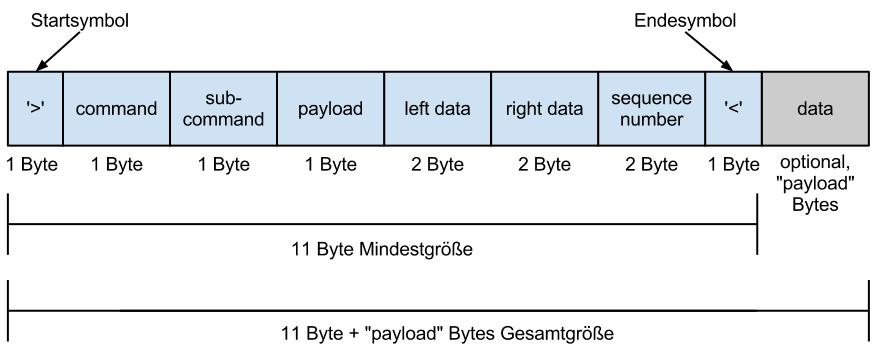
\includegraphics[scale=0.5]{pic/ctBotWlanAllgemein}
	\caption{Allgemeiner Aufbau eines \textit{commands} in einem WLAN-Paket}
	\label{ctBotWlanAllgemein}
\end{figure}


\subsubsection{Auf dem PC}
Um Daten an den Bot zu senden sind lediglich zwei Schritte erforderlich:
\begin{itemize}
	\item Zum WLAN verbinden\\
	Ist der Bot korrekt konfiguriert öffnet er ein Ad-Hoc-WLAN. Zu diesem muss man sich verbinden.
	\item Paket an den Bot senden bzw. Daten empfangen\\
	Ist man mit dem WLAN verbunden kann man einfach ein UDP-Paket mit einen speziellen Inhalt (siehe \ref{wlan_auf_bot}) an den Bot senden, so dass dieser das Paket auswerten kann.\\
	In unserem Fall sieht ein Paket folgendermaßen aus:
	\begin{figure}[H]
		\centering
		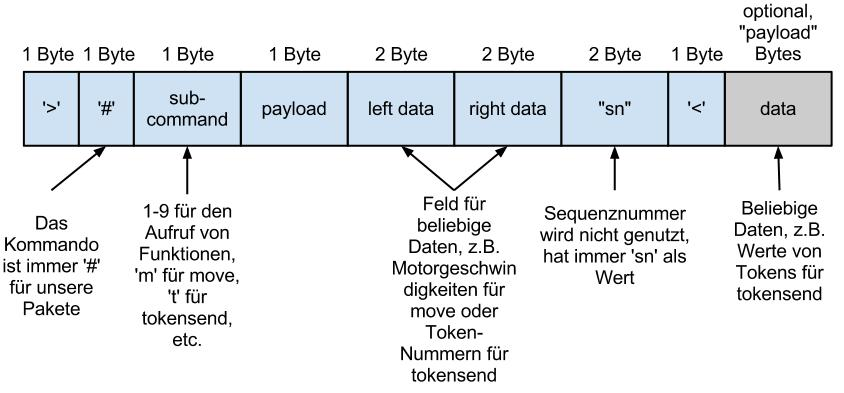
\includegraphics[scale=0.5]{pic/ctBotWlanKonkret}
		\caption{Konkreter Aufbau eines \textit{commands} für unsere Anwendung}
		\label{ctBotWlanKonkret}
	\end{figure}
	
	Hierzu kann z.B. das Tool \textit{sendip} verwendet werden. Ein Beispiel hierzu:\\
	\textit{\$ perl -e 'print "'\textgreater\#\textbackslash x02\textbackslash x06\textbackslash x03\textbackslash x11\textbackslash
    x02\textbackslash x02xy\textless hallo\textbackslash x00"'' \textgreater test.bin\\
    \$ sudo sendip -p ipv4 -is 192.168.0.234 -p udp -us 2000 -ud 10002 -f test.bin 192.168.0.9}\\
    Hierzu wird zunächst mit einem PERL print-Befehl ein Paket erzeugt und in eine Datei geschrieben und anschließen wird der Dateiinhalt mit \textit{sendip} an den Bot (hier 192.168.0.9) gesendet.
	(Die Paramter von links nach rechts: Protokoll IPv4, Quell-IP 192.168.0.234, Protokoll UDP, UDP-Quellport 2000, UDP-Zielport 10002, Datei (deren Inhalt gesendet werden soll) test.bin, die Ziel-IP 192.168.0.9)
	Der Grund für den Umweg über die Datei ist lediglich, dass man sich dadurch "'verlorene"' Zeichen oder kaputte Eingaben erspart, was der Fall wäre wenn man die Eingabe piped oder über eine Subshell erzeugt.
\end{itemize}
Die wesentlich einfachere Variante Pakete an den Bot zu schicken ist das Skript \verb+ctremote.py+ bzw. dessen Funktion \verb+send_cmd(...)+. Dazu siehe \ref{ctremote}.

\subsection{Zusatzaufgabe}

\subsubsection{ctremote.py - Ein Skript zur Fernsteuerung des Bots}
\label{ctremote}
Das Skript ist ein interaktives Programm, welches dem Nutzer ermöglicht Befehle einzugeben, die Aktionen auf Seiten des Bots auslösen. Dazu muss auf dem Bot das Programm laufen, welches in Abschnitt \ref{ctremote_bot} beschrieben ist.\\
Sieht der Nutzer folgenden Prompt, kann er Befehle eingeben:

\textbf{ctBot-remote \$}\\
Nachfolgend die bisher implementierten Befehle:
\begin{itemize}
	\item subcmd <subcommand>\\
	Sendet den angegebenen Subcommand <subcommand> an den Bot. Es sind bisher folgende Subcommands implementiert:
	\begin{itemize}
		\item 1 oder stand\\
		Lässt den Bot anhalten.
   		\item 2 oder motte1\\
   		Lässt den Bot die erste Implementierung von "'Motte"' ausführen.
   		\item 3 oder kakerlake1\\
   		Lässt den Bot die erste Implementierung von "'Kakerlake"' ausführen.
   		\item 4 oder motte2\\
   		Lässt den Bot die zweite Implementierung von "'Motte"' ausführen.
   		\item 5 oder kakerlake2\\
   		Lässt den Bot die zweite Implementierung von "'Kakerlake"' ausführen.
   		\item 6 oder acht\\
   		Lässt den Bot eine Acht fahren.
   		\item 7 oder linie\\
   		Lässt den Bot eine Linie entlang fahren.
	\end{itemize}
	Beispiel: \textit{subcmd motte1}
	
	Beispiel 2 : \textit{subcmd 6}
	\item move\\
	Nach Eingabe dieses Befehls ist der Bot über die Tastatur fernsteuerbar. Die Tastenbelegung dafür ist wie folgt:
	\begin{itemize}
		\item \textbf{W} Vorwärts fahren.
		\item \textbf{S} Rückwärts fahren.
		\item \textbf{A} Nach links drehen.
		\item \textbf{D} Nach rechts drehen.
		\item \textbf{E} Anhalten.
		\item \textbf{Q} Beendet den move-Befehl und kehrt zur Befehlseingabe zurück.
	\end{itemize}
	\item get <what>\\
	Zeigt einem den aktuellen Wert von <what> an. Dabei kann <what> momentan \textit{botip} (also die IP des zu steuernden Bots) oder \textit{port} (also der UDP-Port, über den kommuniziert wird) sein.
	
	Beispiel: \textit{get botip}
	\item set <what> <value>\\
	Setzt den Wert von <what> auf <value>. Hierbei kann <what> wieder \textit{botip} oder \textit{port} sein.
	
	Beispiel: \textit{set botip 192.168.0.9}
	\item help\\
	Gibt einen kurze Übersicht aller Befehle mit einer kurzen Beschreibung aus.
	\item help <cmd>\\
	Gibt einen detaillierten Hilfetext zum angegebenen Befehl <cmd> aus.
	
	Beispiel: \textit{help subcmd}
	\item exit\\
	Beendet das Skript.
	\item quit\\
	Beendet das Skript.
\end{itemize}
Die Tastenkombination \textit{STRG+C} wird von dem Skript abgefangen und sendet dem Bot sofort den Befehl zum Anhalten, beendet das Skript jedoch nicht. Um das Skript zu beenden muss einer der oben beschrieben Befehle \textit{quit} oder \textit{exit} verwendet werden.

\subsubsection{Aufbau von ctremote.py}
Das Skript besteht intern aus folgenden Funktionen:

\begin{itemize}
	\item \verb+help(cmd="")+\\
	Die Funktion bekommt einen optionalen Parameter \textit{cmd}. Wird kein Parameter übergeben, gibt die Funktion einen allgemeinen Hilfetext aus. Wird jedoch ein Befehl als Parameter übergeben, gibt die Funktion eine, für den übergebenen Befehl, passende Hilfe aus.
	\item \verb+openSocket()+\\
	Die Funktion öffnet einen neuen UDP-Socket mit IP und Port der aktuellen Konfiguration. (IP und Port entweder wie im Skript selbst hinterlegt oder mit dem \textit{set}-Befehl (siehe \ref{ctremote}) gesetzt.)
	\item \verb+send_cmd(subcmd,ldata="ld",rdata="rd",payload="\x00",data="")+\\
	Diese Funktion ist dafür zuständig ein Paket nach Norm des Bots (siehe \ref{wlan_auf_bot}) zusammenzubauen und schließlich an ihn zu senden.
	Der einzig zwingend nötige Parameter ist der Subcommand \textit{subcmd} (1 Byte), welcher dem Bot die auszuführende Aktion mitteilt.
	Optionale Parameter sind \textit{ldata} (2Byte) und \textit{rdata} (2 Byte), welche z.B. als Parameter für den Subcommand genutzt werden können, sowie \textit{payload} (1 Byte, Größe von \textit{data}) und \textit{data} (bis zu 255 Byte), welche genutzt werden können, wenn man zusätzliche Daten an den Bot senden will.
	Die Größe der Parameter ist dabei genau einzuhalten.
	\item \verb+recv()+\\
	Diese Funktion läuft während der gesamten Ausführung des Skripts als Thread und ist dafür zuständig Daten vom Bot zu empfangen und zu verarbeiten.
	\item \verb+user_input_eval(usrin)+\\
	Diese Funktion ist dafür zuständig die Eingaben des Nutzers zu interpretieren und die entsprechenden Aktionen durchzuführen, indem sie die anderen Funktionen des Skripts aufruft.
	Der zwingend anzugebende Paramter \textit{usrin} ist dabei die Eingabe des Nutzers.
	\item \verb+move()+
	In dieser Funktion läuft eine Schleife, welche dauerhaft die Tastatureingaben einliest und entsprechend der Eingabe den Bot fahren lässt (wozu sie intern \verb+send_cmd+ nutzt). Die Schleife wird erst duch drücken der Taste Q beendet.
\end{itemize}


\subsubsection{Programm auf dem Bot}
\label{ctremote_bot}
TODO: wie sieht das programm aus, welches die WLAN-pakete auswertet und aktionen auslöst blablabla...


\newpage

% \section{Zeitplan}
% Zeitaufwand aller Projekte (aufgelöst und verrechnet)
% % Zeitaufwand aller Projekte (aufgelöst und verrechnet) als Tabelle

\begin{center}
	\begin{tabular}{  c | c | c | c |}
		\cline{2-4}
		& \multicolumn{3}{|c|}{Zeit}  \\ 
		\hline
		\multicolumn{1}{|c|}{Aufgabe} & Lösungsfindung & Implementierung & Tweaking \\
		\hline
		\hline
		\multicolumn{1}{|c|}{\nameref{benutzung} \ref{benutzung}}  &  &  & \\ 
		\hline
		\multicolumn{1}{|c|}{\nameref{motte_kakerlake} \ref{motte_kakerlake}}  &  &  & \\ 
		\hline
		\multicolumn{1}{|c|}{\nameref{linie_folgen} \ref{linie_folgen}} &  &  & \\ 
		\hline
		\multicolumn{1}{|c|}{\nameref{8-fahren} \ref{8-fahren}} &  &  &\\ 
		\hline
		\multicolumn{1}{|c|}{\nameref{fernsteuerung} \ref{fernsteuerung}} &  &  & \\ 
		\hline
		\multicolumn{1}{|c|}{\nameref{weg-aufzeichnen} \ref{weg-aufzeichnen}} &  &  & \\ 
		\hline
  \end{tabular}
\end{center}



%\section{Quellen}
%\bibliography{doku}{}
%\bibliographystyle{alpha}

\end{document}

